% \documentclass{beamer}
\documentclass[xcolor=dvipsnames]{beamer}
\usefonttheme{serif}
%% \usecolortheme[named=Blue]{structure}
\setbeamersize{text margin left=30mm, text margin right=30mm}
\useoutertheme{infolines}
%% \usetheme[height=7mm]{Rochester}
\usetheme{Pittsburgh}
\setbeamertemplate{items}[ball]
\setbeamertemplate{blocks}[rounded][shadow=true]
\setbeamertemplate{navigation symbols}{}

\usepackage[utf8x]{inputenc}
%% \usepackage{default}
\usepackage[english]{babel}
\usepackage{geometry}
%% \usepackage{fullpage}
\usepackage{amsmath, amsthm, amssymb}
\usepackage{listings}
\usepackage{pxfonts}
\usepackage{caption}

%% \usepackage{color}
%% \usepackage{graphicx}
%% \usepackage{natbib}
%% \usepackage{array}
%% \usepackage{booktabs}
%% \usepackage{tabu}
%% \usepackage[utf8]{inputenc}
%% \usepackage{fancyhdr}
%% \usepackage{float}
%% \usepackage{subfigure}
%% \usepackage{titlesec}

\setbeamertemplate{headline}{}
\setbeamertemplate{footline}[frame number]{}
\setbeamertemplate{navigation symbols}{}
\setbeamertemplate{footline}{}
\setbeamertemplate{footline}[frame number]

\setbeamertemplate{itemize items}{$-$}

\def\CCT{{C\nolinebreak[4]\hspace{-.05em}\raisebox{.4ex}{\tiny\bf ++}}}
\def\CC{{C\nolinebreak[4]\hspace{-.05em}\raisebox{.4ex}{\small\bf ++}}}


\definecolor{lstgray}{gray}{0.93}
\definecolor{strgray}{gray}{0.4}

\lstset{ %
  escapechar=@,
  language=C++,
  basicstyle=\footnotesize\ttfamily,
  %% basicstyle=\ttfamily,
  %% keywordstyle=\color{blue}\ttfamily,
  keywordstyle=\bfseries,
  stringstyle=\color{strgray}\ttfamily,
  commentstyle=\color{OliveGreen}\ttfamily,
  %% morecomment=[l][\color{red}]{\#},
  morecomment=[l][\color{blue}]{\#},
  backgroundcolor=\color{lstgray},
  %% keywordstyle=\color{red},
  frame=f,
  frameround=ffff,
  tabsize=2,
  breaklines=true,
  breakatwhitespace=false,
  showspaces=false,
  showstringspaces=false,
  xleftmargin=5pt,
  xrightmargin=5pt,
  morekeywords={in,out,ref,auto,inout,import,ushort,scope,exit,mixin,decltype,varid,sizeof,constexpr}
}

\def\redcolor{\color{red}}
\def\bluecolor{\color{blue}}
\def\blackcolor{\color{black}}
\def\graycolor{\color{gray}}
\def\greencolor{\color{OliveGreen}}


\def\sectionname{\translate{Section}}
\def\insertsectionnumber{\arabic{section}}
\setbeamertemplate{section page}
{
  \begin{centering}
    \begin{beamercolorbox}[sep=4pt,center]{part title}
      \usebeamerfont{section title}\insertsection\par
    \end{beamercolorbox}
  \end{centering}
}
\def\sectionpage{\usebeamertemplate*{section page}}


\AtBeginSection{\frame{\sectionpage}}


\title{Eight daughters of Lust}
\subtitle{The preeminent role of the intellect}
\author{Dominic Jones}
\date{\small{March 2019}}
\institute{\small{Netherhall House, London}}


\begin{document}
\begin{frame}[plain]
  \titlepage
\end{frame}


\section{``The Moral Obligation To Be Intelligent'', John Erskine}


\begin{frame}[fragile]{“Be good, sweet maid, and let who will be clever”}
  \begin{columns}[T] % align columns
    %% \begin{column}{0.3\textwidth}
    %% \end{column}%
    %% \hfill%
    \begin{column}{0.9\textwidth}
      \begin{figure}[H]
        \centering
        
\includegraphics[width=0.99\textwidth]{wooster}
      \end{figure}
    \end{column}%
  \end{columns}
\end{frame}


\begin{frame}[fragile]{“Revenge. The villainy you teach me I will execute”}
  \begin{columns}[T] % align columns
    %% \begin{column}{0.3\textwidth}
    %% \end{column}%
    %% \hfill%
    \begin{column}{0.9\textwidth}
      \begin{figure}[H]
        \centering
        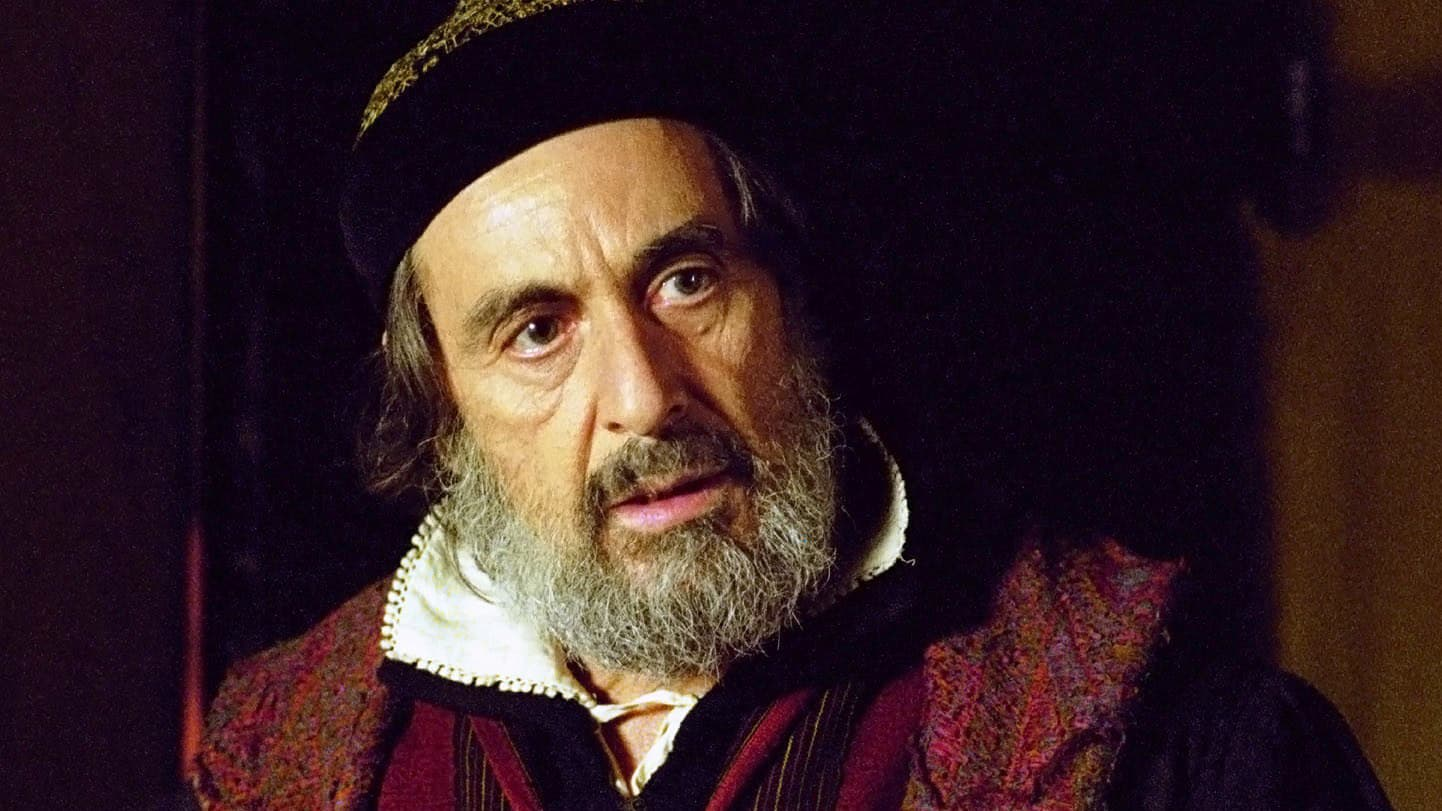
\includegraphics[width=0.99\textwidth]{shylock}
      \end{figure}
    \end{column}%
  \end{columns}
\end{frame}


\section{``The final battle will be about marriage and the family'', Sr. Lucia of Fatima}


\begin{frame}[fragile]{Rearing of children, mutual aid, remedy of concupiscence}
  \begin{columns}[T] % align columns
    %% \begin{column}{0.3\textwidth}
    %% \end{column}%
    %% \hfill%
    \begin{column}{0.8\textwidth}
      \begin{figure}[H]
        \centering
        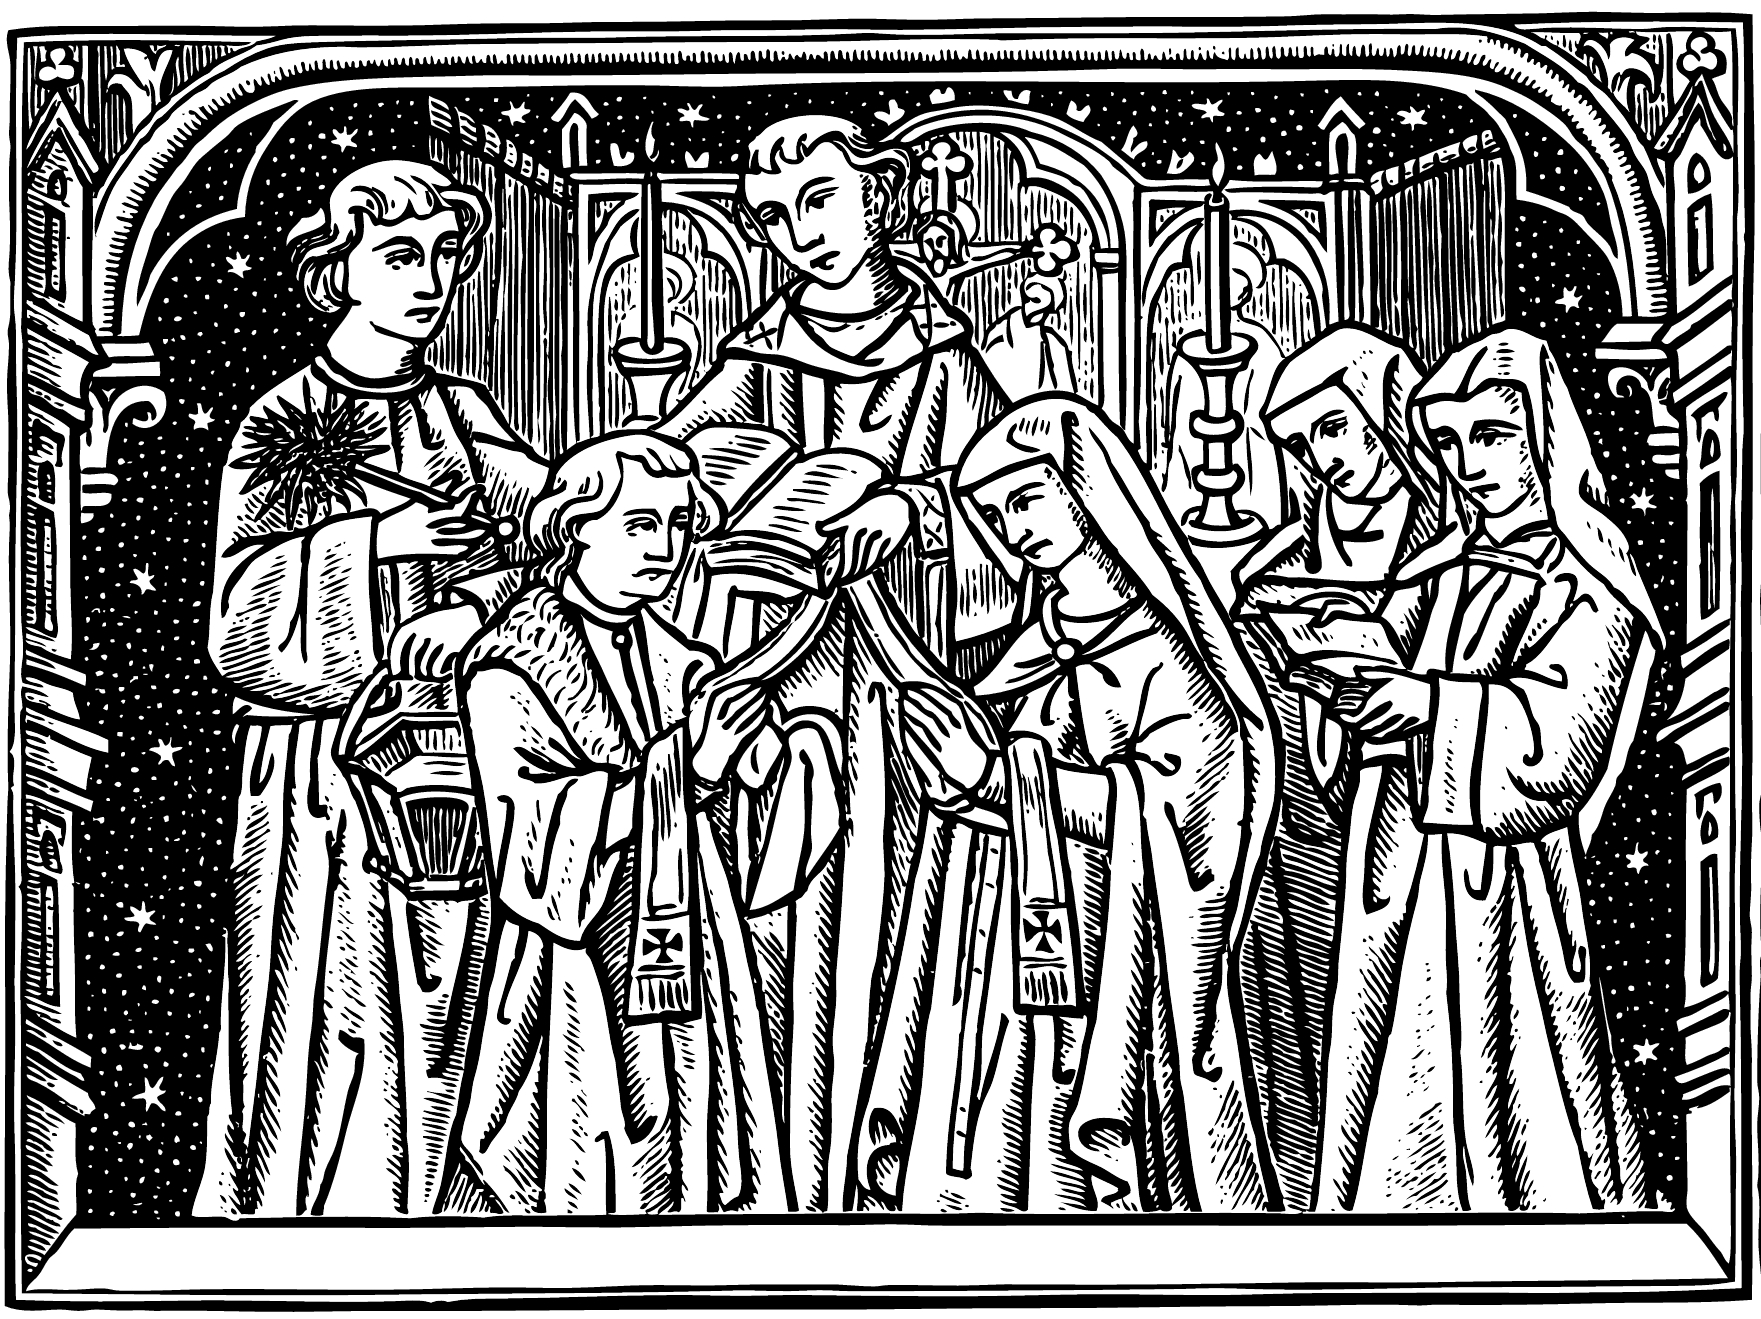
\includegraphics[width=0.99\textwidth]{marriage}
      \end{figure}
    \end{column}%
  \end{columns}
\end{frame}


\section{``What is needed is the cold shower of reason'', E. Feser}


\begin{frame}[fragile]{``I made a mistake. I fell in love. That wasn't part of the plan''}
  \begin{columns}[T] % align columns
    %% \begin{column}{0.3\textwidth}
    %% \end{column}%
    %% \hfill%
    \begin{column}{0.8\textwidth}
      \begin{figure}[H]
        \centering
        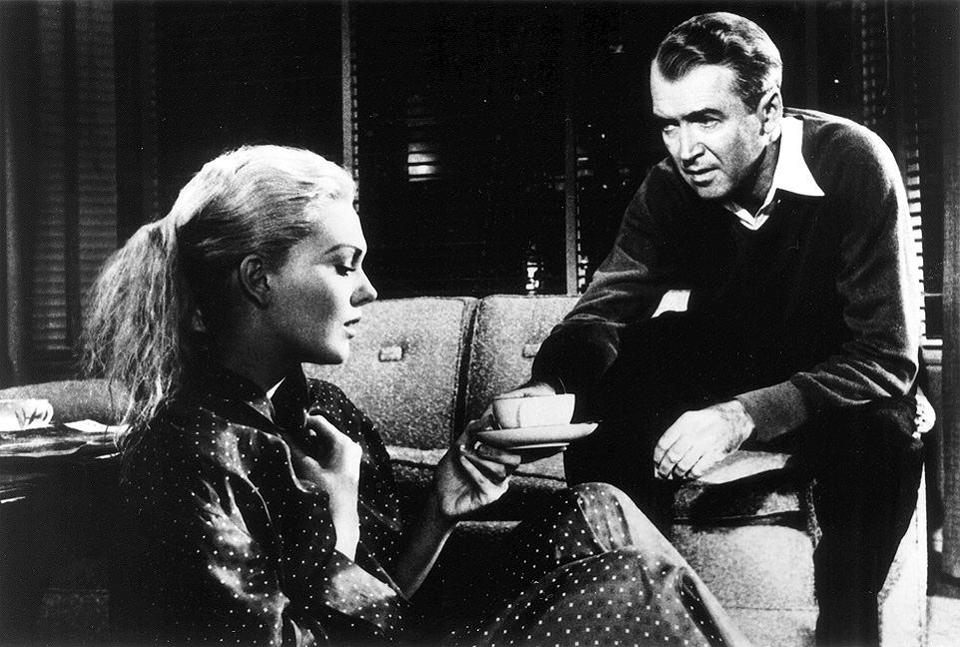
\includegraphics[width=0.99\textwidth]{vertigo}
      \end{figure}
    \end{column}%
  \end{columns}
\end{frame}


\begin{frame}[fragile]{``Scottie’s is an Erotic love of the most rarefied sort''}
  \begin{columns}[T] % align columns
    %% \begin{column}{0.3\textwidth}
    %% \end{column}%
    %% \hfill%
    \begin{column}{0.8\textwidth}
      \begin{figure}[H]
        \centering
        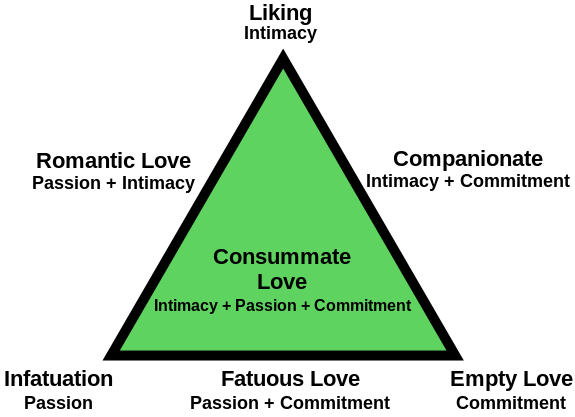
\includegraphics[width=0.99\textwidth]{love}
      \end{figure}
    \end{column}%
  \end{columns}
\end{frame}


\begin{frame}[fragile]{'So long as she's pretty' - Venus}
  \begin{columns}[T] % align columns
    %% \begin{column}{0.3\textwidth}
    %% \end{column}%
    %% \hfill%
    \begin{column}{0.9\textwidth}
      \begin{figure}[H]
        \centering
        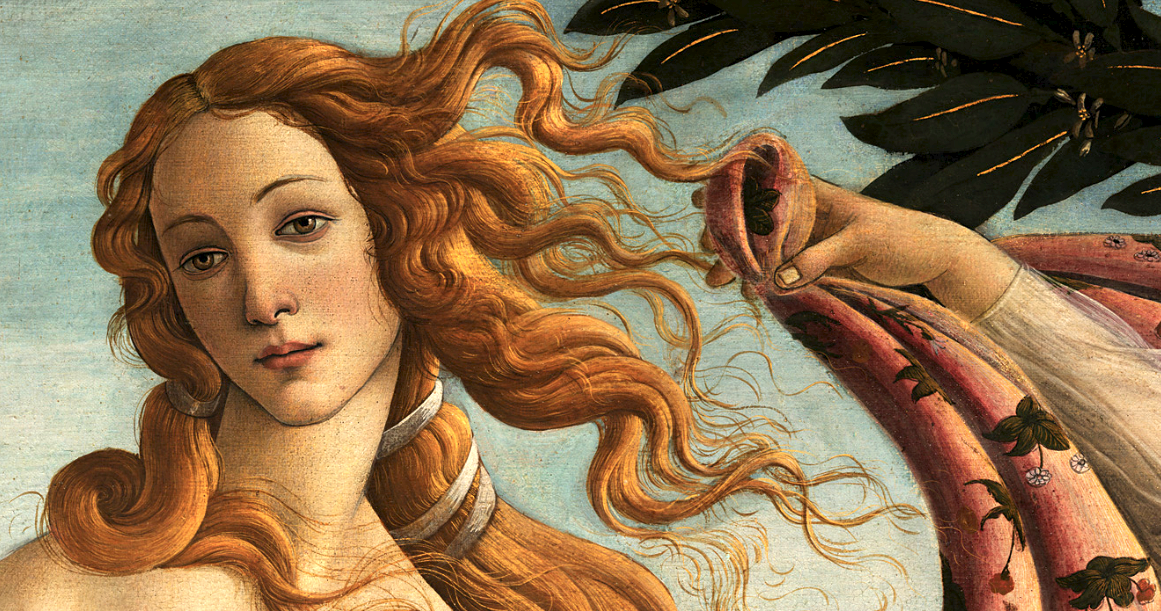
\includegraphics[width=0.99\textwidth]{venus}
      \end{figure}
    \end{column}%
  \end{columns}
\end{frame}


\begin{frame}[fragile]{'No other can satisfy' - Eros}
  \begin{columns}[T] % align columns
    %% \begin{column}{0.3\textwidth}
    %% \end{column}%
    %% \hfill%
    \begin{column}{0.6\textwidth}
      \begin{figure}[H]
        \centering
        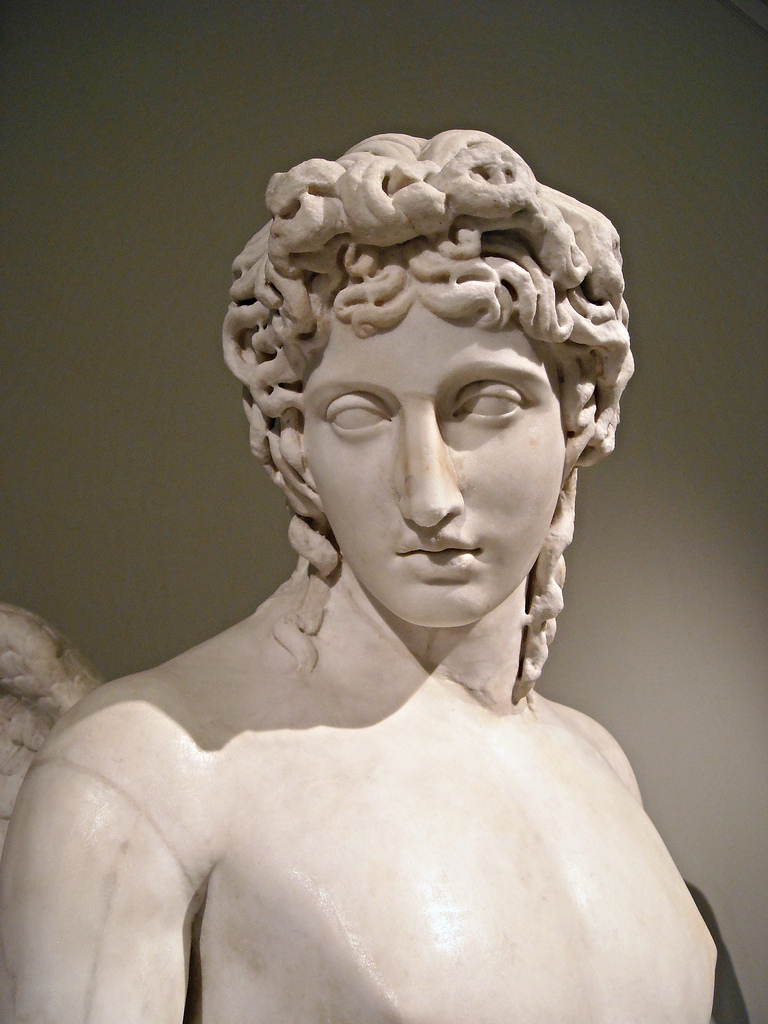
\includegraphics[width=0.99\textwidth]{eros}
      \end{figure}
    \end{column}%
  \end{columns}
\end{frame}


\section{Our highly unusual place in the order of things}


\begin{frame}[fragile]{Angels - Neither sexed nor romantic}
  \begin{columns}[T] % align columns
    %% \begin{column}{0.3\textwidth}
    %% \end{column}%
    %% \hfill%
    \begin{column}{0.8\textwidth}
      \begin{figure}[H]
        \centering
        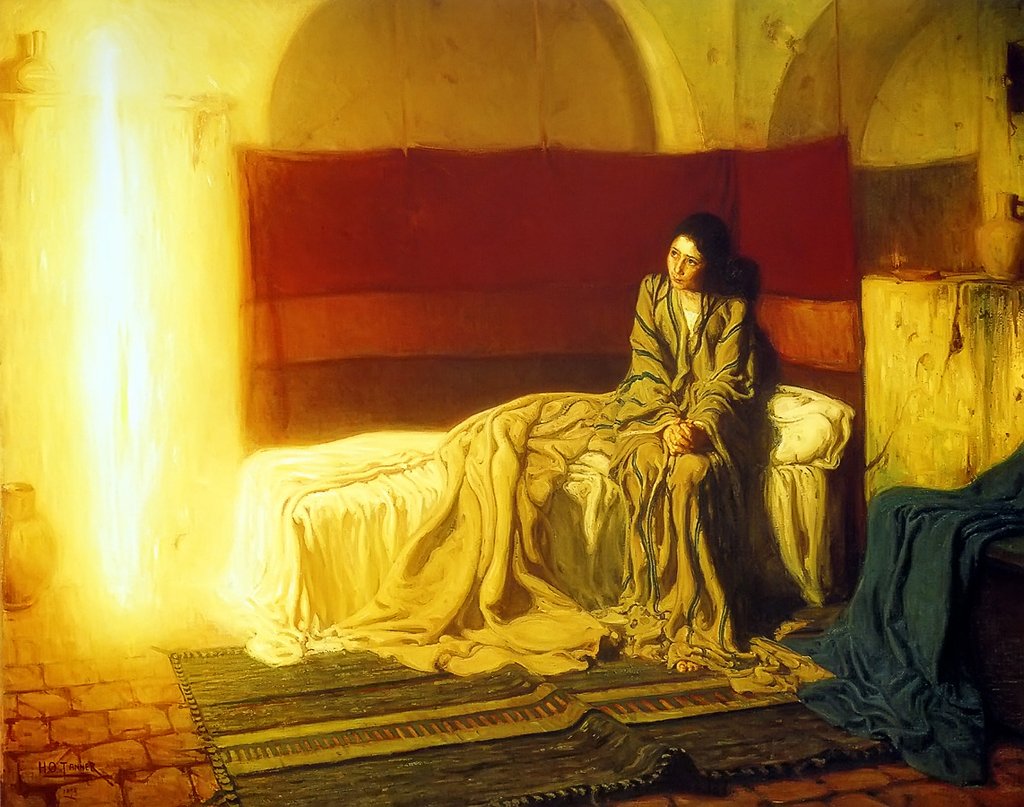
\includegraphics[width=0.99\textwidth]{angel}
      \end{figure}
    \end{column}%
  \end{columns}
\end{frame}


\begin{frame}[fragile]{Animals - Sexed but not romantic}
  \begin{columns}[T] % align columns
    %% \begin{column}{0.3\textwidth}
    %% \end{column}%
    %% \hfill%
    \begin{column}{0.65\textwidth}
      \begin{figure}[H]
        \centering
        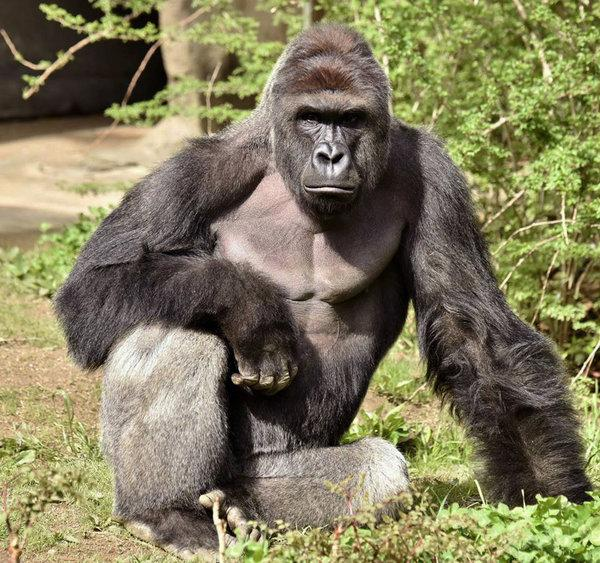
\includegraphics[width=0.99\textwidth]{gorilla}
      \end{figure}
    \end{column}%
  \end{columns}
\end{frame}


\begin{frame}[fragile]{*Sob-Sob* 'It bothers \emph{me} though\ldots'}
  \begin{columns}[T] % align columns
    %% \begin{column}{0.3\textwidth}
    %% \end{column}%
    %% \hfill%
    \begin{column}{0.99\textwidth}
      \begin{figure}[H]
        \centering
        
\includegraphics[width=0.99\textwidth]{buckie}
      \end{figure}
    \end{column}%
  \end{columns}
\end{frame}


\section{``Be fruitful and multiply'', Gn 1:28}


\begin{frame}[fragile]{Nature tells of 'what it's for'}
  \begin{columns}[T] % align columns
    %% \begin{column}{0.3\textwidth}
    %% \end{column}%
    %% \hfill%
    \begin{column}{0.75\textwidth}
      \begin{figure}[H]
        \centering
        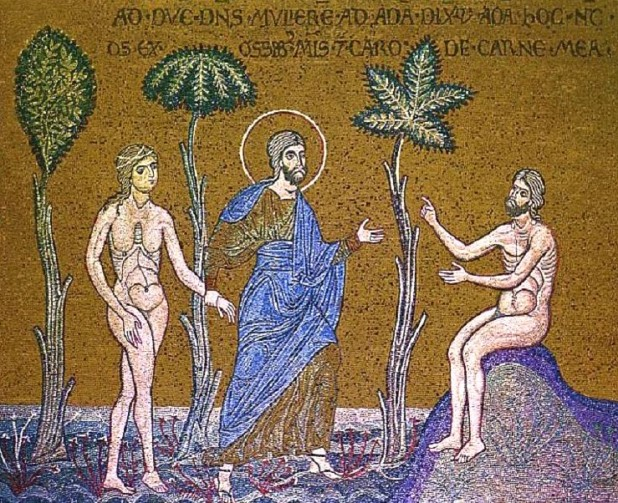
\includegraphics[width=0.99\textwidth]{fruitful}
      \end{figure}
    \end{column}%
  \end{columns}
\end{frame}


\begin{frame}[fragile]{``Quid est veritas?''}
  \begin{columns}[T] % align columns
    %% \begin{column}{0.3\textwidth}
    %% \end{column}%
    %% \hfill%
    \begin{column}{0.9\textwidth}
      \begin{figure}[H]
        \centering
        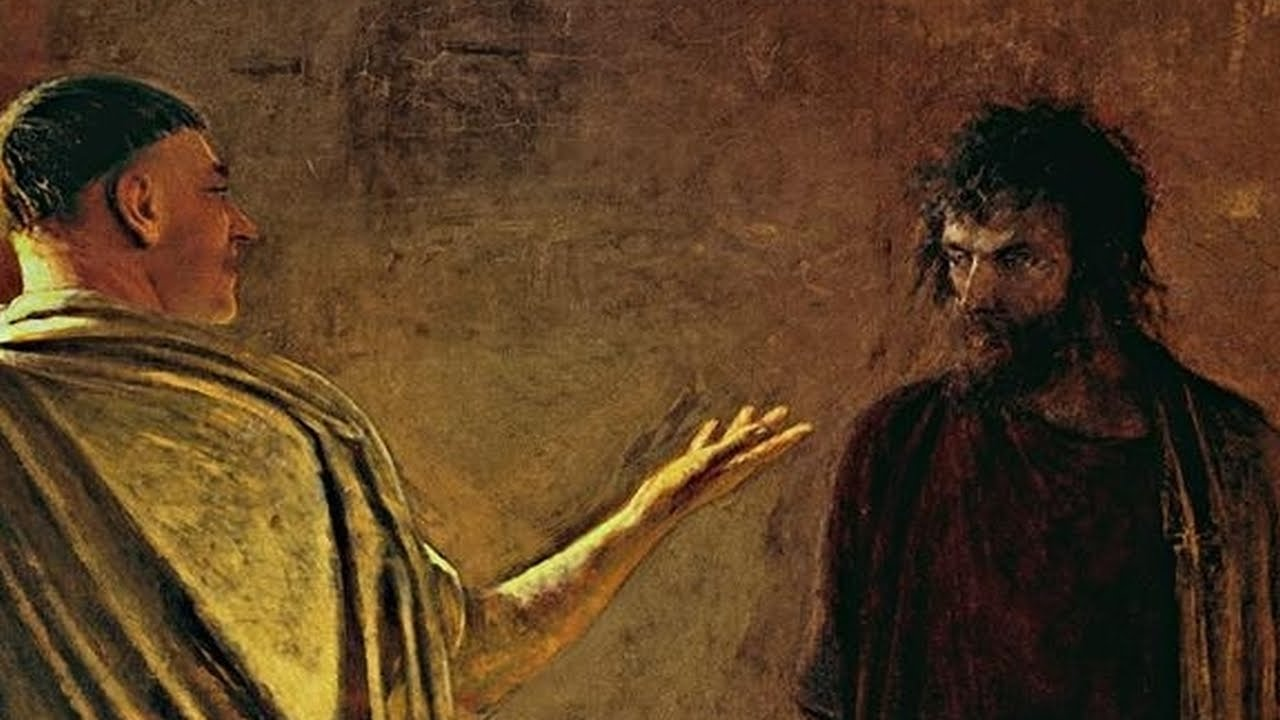
\includegraphics[width=0.99\textwidth]{pilate}
      \end{figure}
    \end{column}%
  \end{columns}
\end{frame}


\section{Blindness of mind, rashness, thoughtlessness, inconstancy}


\section{Self love, hatred of God, love of this world, dispair of the next}


\begin{frame}[plain]
  \titlepage
\end{frame}
\end{document}
